\documentclass[a4paper,11pt]{article}
\usepackage{amssymb}
\usepackage[polish]{babel}
\usepackage[utf8]{inputenc}

\usepackage[T1]{fontenc}
\usepackage{graphicx}
\usepackage{anysize}
\usepackage{enumerate}
\usepackage{times}
\usepackage{geometry}
\usepackage{amsthm}
\usepackage{pgfplots}
\usepackage{amsmath}
\usepackage{mathtools}
\usepackage{amssymb}
\usepackage{multirow}
\usepackage{changepage}
\usepackage{pbox}

\marginsize{3cm}{3cm}{1.5cm}{1.5cm}
\sloppy

\begin{document}
\begin{table}[ht]
\centering
\hspace*{-1cm}
\begin{tabular}{lllllll}
\cline{1-6}
\multicolumn{1}{|c|}{\begin{tabular}[c]{@{}c@{}}EAIiIB\\ Informatyka\end{tabular}}              & \multicolumn{2}{l|}{\begin{tabular}[c]{@{}l@{}}Ewa Stachów\\ Weronika Olcha\end{tabular}}                                                                                                & \multicolumn{1}{c|}{\begin{tabular}[c]{@{}c@{}}Rok\\ II\end{tabular}}          & \multicolumn{1}{c|}{\begin{tabular}[c]{@{}c@{}}Grupa\\ 3\end{tabular}}            & \multicolumn{1}{c|}{\begin{tabular}[c]{@{}c@{}}Zespół\\ 6\end{tabular}}      &  \\ \cline{1-6}
\multicolumn{1}{|c|}{\begin{tabular}[c]{@{}c@{}}Pracownia\\ FIZYCZNA\\ WFiIS AGH\end{tabular}} & \multicolumn{4}{l|}{\begin{tabular}[c]{@{}l@{}}Temat:\\ \textbf{\textit{Współczynnik załamania ciał stałych}} \end{tabular}}                                                                                                                                                                                                                                            & \multicolumn{1}{c|}{\begin{tabular}[c]{@{}c@{}}Nr ćwiczenia:\\ 51\end{tabular}} &  \\ \cline{1-6}
\multicolumn{1}{|l|}{\begin{tabular}[c]{@{}c@{}}Data wykonania:\\ 19.11.2016\end{tabular}}      & \multicolumn{1}{c|}{\begin{tabular}[c]{@{}c@{}}Data oddania:\\ 22.11.2016\end{tabular}} & \multicolumn{1}{l|}{\begin{tabular}[c]{@{}l@{}}Zwrot do poprawki:\\ \phantom{data poprawki}\end{tabular}} & \multicolumn{1}{l|}{\begin{tabular}[c]{@{}l@{}}Data oddania:\\  \phantom{data oddania}\end{tabular}} & \multicolumn{1}{l|}{\begin{tabular}[c]{@{}l@{}}Data zaliczenia:\\  \phantom{data zaliczenia}\end{tabular}} & \multicolumn{1}{l|}{\begin{tabular}[c]{@{}l@{}}OCENA:\\ \phantom{ocena}\end{tabular}}       &  \\ \cline{1-6}
                                                                                               &                                                                                         &                                                                                     &                                                                                &                                                                                   &                                                                               & 
\end{tabular}
\end{table}

\begin{center}
\begin{LARGE}
\textbf{Ćwiczenie nr 51: Współczynnik załamania ciał stałych}
\end{LARGE}
\end{center}

\section{Cel ćwiczenia}
Wyznaczenie współczynnika załamania światła dla ciał stałych metodą mikroskopu. 
Zbadanie zależności współczynnika załamania od długości fali.

\section{Wstęp}
Załamanie światła na granicy dwóch ośrodków przeźroczystych. Promień padający biegnący w~pierwszym ośrodku pada na granicę ośrodków po czym zmienia kierunek, i jako promień złamany biegnie w ośrodku drugim.	
Wiązka światła ulega załamaniu, gdy przechodzi z jednego ośrodka do drugiego o innych własnościach optycznych.
$$
\frac{\sin{\alpha}}{\sin{\beta}} = \frac{V_1}{V_2}
$$
Stosunek sinusa kąta padania do sinusa kąta załamania, zwany współczynnikiem załamania n~ośrodka 2 względem ośrodka 1, jest równy stosunkowi prędkości rozchodzenia się fali w ośrodku 1 do prędkości rozchodzenia się fali w ośrodku 2. W obu ośrodkach promień fali padającej, promień fali załamanej i prosta prostopadła do granicy ośrodków leżą w jednej płaszczyźnie. Prawo załamania zostało sformułowane przez Snelliusa w XVII wieku. \\
$$
n = \frac{\sin{\alpha}}{\sin{\beta}} = \frac{V_1}{V_2} = \frac{n_2}{n_1}
$$
\begin{figure}[ht]
	\centering
	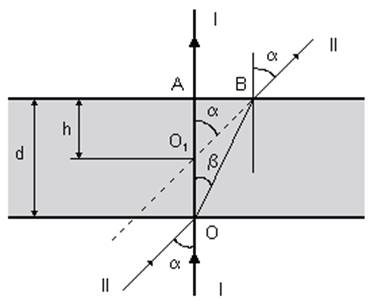
\includegraphics[width=90mm]{image006.jpg}
	\caption{Powstanie  pozornego  obrazu  $O_{1}$ punktu  $O$  leżącego  na  dolnej  powierzchni płytki płaskorównoległej. }
\end{figure}
W skutek załamania wiązki światła odległości przedmiotów umieszczonych w środowisku optycznie gęstszym obserwowane z powietrza wydają się mniejsze. Przykładami mogą być szyba, która wydaje się być cieńsza niż w rzeczywistości lub choćby nawet przedmioty w wodzie, które wydają się być bliżej tafli. Widać to wyraźnie na przykładzie płytki płaskorównoległej:
Promień $OB$ tworzy z prostopadłą wewnątrz szkła kąt $\beta$, a w powietrzu kąt $\alpha$ (wskutek załamania $\alpha > \beta$). Obserwowane promienie, które wychodzą z płytki są rozbieżne, a ich przedłużenia przecinają się w punkcie $O_1$ tworząc obraz pozorny. Rzeczywista grubość płytki to: $d = AO$, natomiast $h = AO_1$ stanowi pozorną grubość płytki płaskorównoległej.


\section{Układ pomiarowy}
\begin{enumerate}
\item Mikroskop wyposażony w czujnik mikrometryczny i nasadkę krzyżową.
\item Śruba mikrometryczna. 
\item Płytka szklana i z pleksiglasu.
\end{enumerate}
\section{Wyniki pomiarów}

	\begin{adjustwidth}{-1cm}{}
\def\arraystretch{1.3}
\begin{center}
	\begin{tabular}{|c|c|c|c|c|}
		\hline
		\multicolumn{5}{|l|}{\begin{tabular}{l} Materiał: pleksiglas\\ Grubość rzeczywista: $d =5,42$ [mm]\\ niepewność $u(d)=0,01$ [mm] \end{tabular}}\\
		\hline
		\multirow{3}{*}{Lp.} & \multicolumn{2}{|c|}{Wskazanie czujnika} & \begin{tabular}{c}Grubość \\pozorna\end{tabular} &\begin{tabular}{c}Współczynnik \\załamania\end{tabular} \\ \cline{2-5}
		& \parbox[c]{1.8 cm}{\centering $a_{d}$}  & $a_{g}$ & $h=a_{d}-a_{g}$ & \multirow{2}{*}{$n=\frac{d}{h}$}\\ \cline{2-4}
		& [mm] & [mm] & [mm] & \\ 
		
		\hline
		1. & 7,75 & 4,21& 3,54& 1,53\\
		\hline
		2. & 7,69 & 4,18& 3,51& 1,54\\
		\hline
		3. & 7,71 & 4,19& 3,52& 1,54\\
		\hline
		4. & 7,76 & 4,22& 3,54& 1,53\\
		\hline
		5. & 7,72 & 4,19& 3,53& 1,54\\
		\hline
		6. & 7,71 & 4,21& 3,50& 1,55\\
		\hline
		7. & 7,74 & 4,17& 3,57& 1,52\\
		\hline
		8. & 7,68 & 4,24& 3,44& 1,58\\
		\hline
		9. & 7,77 & 4,26& 3,51& 1,54\\
		\hline
		10.& 7,70 & 4,19& 3,51& 1,54\\
		\hline
		\multicolumn{2}{c|}{}&\begin{tabular}{c}Wartość \\ średnia \end{tabular}&3,51 &1,54 \\
		\cline{3-5}
		\multicolumn{2}{c|}{}&\begin{tabular}{c}Niepewność \end{tabular}& 0,63& 0,12\\
		\cline{3-5}
	\end{tabular}
	\end{center}
\end{adjustwidth}


\begin{adjustwidth}{-1cm}{}
\def\arraystretch{1.3}
\begin{center}
	\begin{tabular}{|c|c|c|c|c|}
		\hline
		\multicolumn{5}{|l|}{\begin{tabular}{l} Materiał: szkło\\ Grubość rzeczywista: $d =4,29$ [mm]\\ niepewność $u(d)=0,01$ [mm] \end{tabular}}\\
		\hline
		\multirow{3}{*}{Lp.} & \multicolumn{2}{|c|}{Wskazanie czujnika} & \begin{tabular}{c}Grubość \\pozorna\end{tabular} &\begin{tabular}{c}Współczynnik \\załamania\end{tabular} \\ \cline{2-5}
		& \parbox[c]{1.8 cm}{\centering $a_{d}$}  & $a_{g}$ & $h=a_{d}-a_{g}$ & \multirow{2}{*}{$n=\frac{d}{h}$}\\ \cline{2-4}
		& [mm] & [mm] & [mm] & \\ 
		
		\hline
		1. & 8,10 & 5,46& 2,64& 1,63\\
		\hline	
		2. & 8,07 & 5,51& 2,56& 1,68\\
		\hline
		3. & 8,04 & 5,59& 2,45& 1,75\\
		\hline
		4. & 8,06 & 5,53& 2,53& 1,70\\
		\hline
		5. & 8,04 & 5,49& 2,55& 1,68\\
		\hline
		6. & 8,04 & 5,48& 2,56& 1,68\\
		\hline
		7. & 8,02 & 5,49& 2,53& 1,70\\
		\hline
		8. & 8,04 & 5,53& 2,51& 1,71\\
		\hline
		9. & 8,04 & 5,53& 2,51& 1,71\\
		\hline
		10.& 8,04 & 5,53& 2,51& 1,71\\
		\hline
		\multicolumn{2}{c|}{}&\begin{tabular}{c}Wartość \\ średnia \end{tabular}&2,54 &1,69 \\
		\cline{3-5}
		\multicolumn{2}{c|}{}&\begin{tabular}{c}Niepewność \end{tabular}& 0,53& 0,12\\
		\cline{3-5}
	\end{tabular}
	\end{center}
\end{adjustwidth}
	
\section{Obliczenia}
Aby obliczyć wartość współczynnika załamania światła korzystamy ze wzoru:
$$n=\frac{d}{h}$$
Niepewność pomiaru grubości płytki typu B przyjmujemy:
$$u(d)=0,01~mm,$$
gdyż jest to najmniejsza możliwa do odczytania wartość na śrubie mikrometrycznej.\\
Do obliczenia niepewności typu A dla grubości pozornej $h$ korzystamy ze wzoru:
$$u(h) = \sqrt{\frac{\sum(h_{i}-\overline{h})^{2}}{n(n-1)}}$$
\textbf{Dla pleksiglasu:}
$$u(h)=\displaystyle \sqrt{\frac{(3,54-3,51)^{2}+\cdots +(3,51-3,51)^{2}}{10(10-1)}}~mm= 0,63~mm$$
\textbf{Dla szkła:}
$$u(h)=\displaystyle \sqrt{\frac{(2,64-2,54)^{2}+\cdots +(2,51-2,54)^{2}}{10(10-1)}}~mm= 0,53~mm$$	
Następnie wyznaczamy niepewność obliczonego współczynnika załamania światła z prawa przenoszenia niepewności:
$$ u(n) =\sqrt{\bigg(\frac{\partial n}{\partial d}u(d)\bigg)^2+\bigg(\frac{\partial n}{\partial h}u(h)\bigg)^2} = \sqrt{\bigg(\frac{1}{h}u(d)\bigg)^2+\bigg(\frac{-d}{h^2}u(h)\bigg)^2}$$
\textbf{Dla pleksiglasu:}
$$ u(n) = \sqrt{\bigg(\frac{1}{3,51}\cdot 0,01\bigg)^2+\bigg(\frac{-7,72} {3,51^2}\cdot 0,63\bigg)^2} = 0,12$$
\textbf{Dla szkła:}
$$ u(n) = \sqrt{\bigg(\frac{1}{2,54}\cdot 0,01\bigg)^2+\bigg(\frac{-8,05} {2,54^2}\cdot 0,53\bigg)^2} = 0,12$$
\section{Porównanie z wartościami tabelarycznymi}
\textbf{Dla pleksiglasu:}
$$u_{tab} = 1,9$$
$$|u_{tab}-u_{obl}|=|1,49-1,54|<u(n)$$ 
\textbf{Dla szkła:}
$$u_{tab} = [1,4;1,9]$$
$$u_{obl} \in [1,4;1,9]$$
\section{Wnioski}
Otrzymane wartości współczynnika załamania są zgodna z wartościami tablicowymi w granicach niepewności zarówno dla płytki ze szkła, jak i z pleksiglasu.
Według przeprowadzonego badania, współczynnik załamania światła w szkle jest mniejszy od współczynnika załamania w plexiglasie -- wynika z~tego, że obraz widziany przez szkło jest wyraźniejszy niż ten widziany przez płytkę z~plexiglasu.  
\end{document}